\chapter[Contexto de Serie de Fourier
]{Contexto de Serie de Fourier}
{
\parindent0pt

Según \cite{Arenas2014}, el estudio de las series de Fourier se originó en los trabajos de Joseph Fourier sobre la propagación del calor en cuerpos sólidos. En 1807, presentó su memoria \textit{Mémoire sur la propagation de la chaleur dans les corps solides}, donde analizaba la evolución de la temperatura en función del tiempo. Su trabajo fue clave para el desarrollo de la teoría del análisis de Fourier, que posteriormente consolidó en 1822 con la publicación de \textit{Théorie analytique de la chaleur}, estableciendo los principios para la expansión en series de funciones trigonométricas que representan fenómenos periódicos.
\vspace{10pt}

\begin{figure}[H]
    \centering
    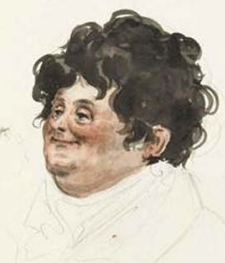
\includegraphics[height=0.15\textheight]{Figures/retrato.png}
    \caption[Retrato caricaturesco de J. Fourier, atribuido a Julien Leopold Boilly]{Retrato caricaturesco de J. Fourier, atribuido a Julien L. Imagen tomada de  \cite{Arenas2014}}
    \label{fig:retrato}
\end{figure}

Las Series de Fourier constituyen una herramienta fundamental en el análisis de funciones, permitiendo representar funciones periódicas como una suma infinita de senos y cosenos. Su estudio se basa en la construcción del espacio \(L^2\) y en la determinación de los coeficientes que conforman la serie. Además, su aplicación se extiende a funciones no periódicas mediante técnicas de extensión y generalización a períodos arbitrarios \citep{DiagoNanez2023}.

\section{Forma Compleja de la Serie de Fourier}
La serie de Fourier puede expresarse en su forma compleja, lo que resulta conveniente en contextos que requieren trabajar con números complejos y simplifica el uso de la Transformada de Fourier \cite{DiagoNanez2023}.  En esta notación, una función \(f(x)\) periódica con período \(T\) se representa como:

\begin{equation} f(x) = \sum_{n=-\infty}^{\infty} c_n e^{i n x}, \end{equation}
\vspace{10pt}

Los coeficientes \(c_n\) se determinan mediante la integral:

\begin{equation} c_n = \frac{1}{T} \int_T f(x) e^{-i n x} , dx \end{equation}

Esta forma compleja de la serie de Fourier permite una interpretación más directa en términos de números complejos y resulta fundamental para la formulación de la Transformada de Fourier \cite{Oppenheim1999, DiagoNanez2023}.

\section{Fórmula Trigonométrica de la Serie de Fourier}

El problema consiste en, dada una función \( f \) de período \( 2\pi \), encontrar su representación en forma de una serie trigonométrica, como se describe en \cite{Arenas2014}. La Serie de Fourier para una función \( f(x) \) en el intervalo \( [-\pi, \pi] \) se expresa de la siguiente manera:

\begin{equation}
\label{eq:fourier}
f(x) = A + \sum_{n=1}^{\infty} a_n \cos(nx) + b_n \sin(nx), \quad \forall x \in T
\end{equation}

En esta ecuación, los coeficientes \( a_0 \), \( a_n \) y \( b_n \) se determinan mediante integrales sobre el intervalo \( T \). Esta representación permite expresar la función \( f(x) \) como una suma infinita de funciones trigonométricas, lo cual facilita el análisis de funciones periódicas.

Los coeficientes \( a_0 \), \( a_n \) y \( b_n \) se calculan mediante las siguientes integrales:
\vspace{10pt}

Coeficiente \( a_0 \):

\begin{equation}
\label{eq:a0Variable}
a_0 = \frac{2}{T} \int_T f(x) \, dx
\end{equation}
\vspace{10pt}

Coeficientes \( a_n \) y \( b_n \):
\vspace{10pt}

\begin{equation}
\label{eq:anVariable}
a_n = \frac{2}{T} \int_T f(x) \cos\left( \frac{2\pi n}{T} x \right) \, dx
\end{equation}

\vspace{10pt}
y
\vspace{10pt}
\begin{equation}
\label{eq:bnVariable}
b_n = \frac{2}{T} \int_T f(x) \sin\left( \frac{2\pi n}{T} x \right) \, dx
\end{equation}
\vspace{10pt}

El procedimiento para obtener el coeficiente \( a_0 \) en la forma trigonométrica de la Serie de Fourier, a partir de la ecuación \eqref{eq:fourier}, es el siguiente. Al integrar esta expresión sobre el intervalo \( T \), y aplicar las propiedades de ortogonalidad de los senos y cosenos, se obtiene:

\[
\int_T f(x) \, dx = \int_T A \, dx + \int_T \sum_{n=1}^{\infty} a_n \cos(nx) + b_n \sin(nx) \, dx 
\]

\begin{equation}
= A \cdot 2\pi + \sum_{n=1}^{\infty} a_n \underbrace{\int_T \cos(nx) \, dx}_{0} + b_n \underbrace{\int_T \sin(nx) \, dx}_{0}
\end{equation}

\[
= A \cdot 2\pi.
\]

Finalmente, tomando \( A = \frac{a_0}{2} \), se obtiene el valor de \( a_0 \) como:

\begin{equation}
a_0 = \frac{1}{\pi} \int_T f(x) \, dx.
\end{equation}
\vspace{10pt}

Para obtener los coeficientes \( a_n \) y \( b_n \), el proceso es análogo. Consiste en multiplicar la ecuación \eqref{eq:fourier} por \( \cos(kx) \) y \( \sin(kx) \), respectivamente, e integrar sobre el intervalo \( T \). Para una derivación detallada de estos coeficientes y una discusión más profunda sobre las series de Fourier, se recomienda consultar \cite{DiagoNanez2023}.

\section{Aplicaciones de la Serie de Fourier}

El análisis de Fourier es una herramienta fundamental en matemáticas e ingeniería, utilizada para descomponer funciones en una suma infinita de senos y cosenos. En particular, la serie de Fourier permite representar funciones periódicas mediante combinaciones de funciones trigonométricas, lo que facilita su estudio y aplicación en diversas áreas del conocimiento \cite{Oppenheim1999}.
\vspace{10pt}

A lo largo de los años, la serie de Fourier ha demostrado ser una herramienta esencial en la resolución de problemas donde la periodicidad y la descomposición en frecuencias juegan un papel clave. Su utilidad se extiende más allá del análisis matemático, permitiendo modelar fenómenos físicos y optimizar procesos en ingenierías. 
\vspace{10pt}

Gracias a su capacidad para transformar funciones complejas en combinaciones de términos sinusoidales, esta técnica se ha convertido en un pilar en múltiples disciplinas.



\subsection{Aplicación en la ciencia}

La serie de Fourier es una herramienta matemática fundamental en las áreas de la ciencia como se muestra a continucación.
\vspace{10pt}

En mecánica cuántica, la serie de Fourier es fundamental para resolver la ecuación de Schrödinger en sistemas periódicos. Su aplicación permite describir la evolución temporal de partículas en potenciales periódicos, como en los cristales cuánticos y los superconductores \cite{griffiths2018introduction}. Además, la transformada de Fourier es utilizada en la representación de estados cuánticos en diferentes bases, lo que facilita la simulación de sistemas cuánticos complejos en computación cuántica \cite{nielsen2010quantum}.
\vspace{10pt}

En astronomía, la serie de Fourier se emplea en la espectroscopia astronómica para descomponer la luz de estrellas y galaxias en componentes espectrales. Esto permite identificar la composición química de cuerpos celestes y analizar efectos como el desplazamiento Doppler en exoplanetas \cite{bracewell2003fourier}. 
\vspace{10pt}

En la radioastronomía, la transformada de Fourier es utilizada en la síntesis de imágenes obtenidas por interferometría, lo que ha permitido la observación de agujeros negros y la detección de ondas gravitacionales \cite{thompson2017interferometry}.
\vspace{10pt}

En ciencia de materiales, la serie de Fourier se aplica en el estudio de estructuras cristalinas. Mediante la difracción de rayos X, los científicos pueden analizar patrones de interferencia que se traducen en series de Fourier para determinar la disposición atómica en materiales sólidos. Esto es esencial para el diseño de nuevos materiales con propiedades específicas, como superconductores o aleaciones de alta resistencia \cite{cullity2014elements}.

En la física, la serie de Fourier es ampliamente utilizada para resolver ecuaciones diferenciales que describen sistemas oscilatorios y ondulatorios. Por ejemplo, en mecánica cuántica, la transformada de Fourier permite representar funciones de onda en el espacio de momentos, lo que es esencial para estudiar partículas en potenciales periódicos, como en los cristales y superconductores \cite{griffiths2018introduction}.
\vspace{10pt}

En la química, la serie de Fourier se utiliza en espectroscopía para analizar las frecuencias de vibración de moléculas. Esto es clave para identificar compuestos químicos y estudiar sus propiedades dinámicas, como en la espectroscopía infrarroja y Raman \cite{banwell1994fundamentals}.


\subsection{Aplicación en la tecnología}

La serie de Fourier es una herramienta matemática en áreas de la tecnología. Sirve para analizar señales en el dominio de la frecuencia y permite optimizar sistemas de telecomunicaciones, mejora la compresión de imágenes y audio, y desarrollar algoritmos en el procesamiento de señales digitales. 
\vspace{10pt}

En el campo de las telecomunicaciones, la serie de Fourier sirve para la modulación y transmisión de señales. Se emplea en técnicas como la multiplexación por división de frecuencia (FDM) y la modulación por división de frecuencia ortogonal (OFDM), utilizadas en sistemas de comunicación inalámbrica como 4G, 5G y Wi-Fi \cite{proakis2001digital}.
\vspace{10pt}

Las series de Fourier también juegan un papel clave en el procesamiento de imágenes digitales. La transformada de Fourier se utiliza en la compresión de imágenes, como en el estándar JPEG, donde permite representar imágenes en términos de sus componentes de frecuencia y eliminar información redundante \cite{gonzalez2017digital}.
\vspace{10pt}

En el campo de la tecnología de audio, la serie de Fourier se utiliza para analizar y procesar señales de sonido. Por ejemplo, en la compresión de archivos de audio (como MP3), la transformada de Fourier permite descomponer la señal en sus componentes frecuenciales, lo que facilita la eliminación de frecuencias no perceptibles por el oído humano y, por tanto, reduce el tamaño del archivo sin perder calidad apreciable \cite{oppenheim2010discrete}.
\vspace{10pt}

En el ámbito de la tecnología médica, la serie de Fourier se aplica en dispositivos de diagnóstico por imagen, como los escáneres de resonancia magnética (MRI). Aquí, la transformada de Fourier convierte las señales captadas en el dominio de la frecuencia en imágenes detalladas del cuerpo humano, lo que permite diagnósticos más precisos y no invasivos \cite{haacke2014magnetic}.
\vspace{10pt}

En la tecnología de energía, la serie de Fourier es fundamental para el análisis de señales en sistemas de potencia. Permite identificar y corregir distorsiones armónicas en la red eléctrica, lo que mejora la calidad de la energía y previene fallos en equipos sensibles \cite{mcgranghan2017power}.

\subsection{Aplicación en la ingeniería}

La serie de Fourier es una herramienta matemática para diversas ramas de la ingeniería. Su capacidad para descomponer señales y analizar su comportamiento en el dominio de la frecuencia mejora el diseño y optimización de sistemas en ingeniería eléctrica, mecánica, civil y biomédica.
\vspace{10pt}

En ingeniería eléctrica, la serie de Fourier se utiliza para analizar y diseñar circuitos de corriente alterna (CA). La representación de señales en el dominio de la frecuencia facilita el estudio del comportamiento de filtros eléctricos, amplificadores y sistemas de comunicación \cite{haykin2001communication}
\vspace{10pt}

En ingeniería mecánica, la serie de Fourier es fundamental en el estudio de vibraciones y el análisis modal de estructuras. Se utiliza para modelar y predecir el comportamiento dinámico de componentes mecánicos sometidos a cargas periódicas, como ejes rotativos, turbinas y motores \cite{inman2001engineering}
\vspace{10pt}

En ingeniería biomédica, la serie de Fourier es esencial para el procesamiento de señales fisiológicas, como electrocardiogramas (ECG) y electroencefalogramas (EEG). Permite la eliminación de ruido en registros médicos y la detección de anomalías en señales biológicas \cite{metin2004biomedical}
\vspace{10pt}

En ingeniería de control, la serie de Fourier es fundamental para el análisis de sistemas dinámicos. Por ejemplo, en el diseño de controladores para robots o vehículos autónomos, la transformada de Fourier ayuda a analizar la respuesta en frecuencia del sistema, lo que permite optimizar su estabilidad y rendimiento \cite{ogata2010modern}.
\vspace{10pt}

En ingeniería civil, la serie de Fourier se utiliza para analizar cargas dinámicas en estructuras, como puentes y edificios. Al estudiar las frecuencias de las fuerzas aplicadas, los ingenieros pueden predecir cómo responderá la estructura a terremotos o vientos fuertes, lo que ayuda a mejorar su diseño y seguridad \cite{chopra2017dynamics}.


\subsection{Aplicación en la Inteligencia Artificial}

La serie de Fourier se ha utilizado en diversos campos, incluida la Inteligencia Artificial. Esto puede ser útil en aplicaciones como el reconocimiento de patrones, el procesamiento de imágenes y la optimización de modelos.
\vspace{10pt}

Las Redes Implícitas Neuronales (INR) utilizan perceptrones multicapa para representar funciones de alta frecuencia en dominios de baja dimensión. Recientemente, estas representaciones han logrado resultados destacados en tareas relacionadas con objetos y escenas 3D complejas \cite{benbarka2021seeing}.
\vspace{10pt}

El análisis armónico, que incluye las series de Fourier, se utiliza para comprender cómo las redes neuronales profundas aprenden tareas complejas. Por ejemplo, investigadores de la Universidad de Rice entrenaron una red neuronal profunda para reconocer flujos complejos de aire o agua y predecir sus cambios en el tiempo \cite{choi2023matematicas}.
\vspace{10pt}

Además, las series de Fourier son esenciales en el procesamiento de señales dentro de la IA, permitiendo la eliminación de ruido, la detección de patrones y la mejora de la calidad de las señales \cite{Oppenheim1999}. Esta técnica es clave en aplicaciones como el reconocimiento de voz, la visión por computadora y la bioinformática, donde la extracción de características relevantes en el dominio de la frecuencia mejora la precisión de los modelos de aprendizaje automático.
\vspace{10pt}

En el análisis de series temporales, la serie de Fourier es empleada para descomponer datos en componentes frecuenciales, lo que ayuda a identificar tendencias y patrones periódicos. Esto es especialmente útil en aplicaciones de predicción, como el pronóstico del tiempo o la detección de anomalías en datos financieros \cite{box2015time}.
\vspace{10pt}

En el aprendizaje profundo (deep learning), la transformada de Fourier se utiliza para acelerar operaciones de convolución en redes neuronales convolucionales (CNN). Aplicando la transformada rápida de Fourier (FFT), es posible reducir la complejidad computacional de estas operaciones, lo que permite entrenar modelos más grandes y complejos de manera eficiente \cite{goodfellow2016deep}.
\vspace{10pt}

En la optimización de modelos de IA, la serie de Fourier se utiliza para analizar y suavizar funciones de pérdida. Esto ayuda a identificar mínimos globales en lugar de mínimos locales, lo que mejora la convergencia de algoritmos de optimización como el descenso de gradiente \cite{boyd2004convex}.


\subsection{Aplicación en el cómputo paralelo}

El cómputo paralelo permite acelerar la ejecución de algoritmos dividiendo tareas en múltiples unidades de procesamiento. La serie de Fourier, junto con su transformada rápida (FFT), es ampliamente utilizada en la optimización de estos algoritmos, reduciendo el tiempo de cómputo en problemas como el análisis de señales, la dinámica de fluidos computacional (CFD) y la inteligencia artificial \cite{vanloan1992computational}.
\vspace{10pt}

En visión por computadora, la serie de Fourier se utiliza para mejorar la eficiencia del procesamiento de imágenes mediante filtrado en el dominio de la frecuencia. La implementación de algoritmos FFT en GPU (Unidades de Procesamiento Gráfico) permite acelerar la detección de bordes, el reconocimiento de patrones y la compresión de imágenes \cite{moreland2003fft}.
\vspace{10pt}

En simulaciones numéricas, como en la dinámica de fluidos computacional (CFD), la serie de Fourier se emplea para resolver ecuaciones en diferencias finitas y para modelar turbulencias \cite{canuto2006spectral}.

\vspace{10pt}

En la optimización de algoritmos paralelos, la serie de Fourier se emplea para diseñar técnicas de descomposición de problemas en subproblemas independientes que pueden resolverse en paralelo. Esto es especialmente útil en aplicaciones de aprendizaje automático distribuido, donde la FFT se utiliza para acelerar operaciones matriciales y de convolución en grandes redes neuronales \cite{goodfellow2016deep}.
\vspace{10pt}

En el análisis de big data, la transformada de Fourier se aplica en el procesamiento paralelo de grandes conjuntos de datos temporales o espaciales. Por ejemplo, en astronomía, la FFT se utiliza para analizar señales de telescopios de manera distribuida, lo que permite procesar petabytes de datos en tiempo récord \cite{bracewell2003fourier}.

\section{Teoría de Procesos Hijos con la Llamada al Sistema fork() en Lenguaje C}

En sistemas operativos basados en UNIX, la llamada al sistema fork() es un mecanismo fundamental para la creación de procesos. Esta función permite a un proceso existente (proceso padre) crear una copia casi idéntica de sí mismo (proceso hijo), estableciendo así un modelo de concurrencia que ha sido esencial en el desarrollo de aplicaciones multiproceso. La naturaleza de fork() establece que, tras su invocación, dos procesos separados continúan la ejecución del programa: el proceso original y su copia recién creada \cite{stevens2013advanced}.
\vspace{10pt}

La singularidad de fork() radica en su comportamiento único de retorno: cuando es invocada correctamente, devuelve dos valores diferentes simultáneamente. En el proceso padre, retorna el identificador del proceso hijo (PID) recién creado, mientras que en el proceso hijo devuelve cero. Este mecanismo permite que ambos procesos determinen su rol y ejecuten código específico según su identidad. Si la llamada a fork() falla, retorna un valor negativo al proceso padre, indicando el error ocurrido \cite{kerrisk2010linux}.
\vspace{10pt}

Durante la creación del proceso hijo, el sistema operativo realiza una duplicación del espacio de memoria del proceso padre, incluyendo variables, descriptores de archivo y otros recursos. Sin embargo, esta duplicación implementa una estrategia de "copia en escritura" (copy-on-write), donde los segmentos de memoria realmente se duplican solo cuando uno de los procesos intenta modificarlos. Esta optimización mejora significativamente el rendimiento de la creación de procesos, especialmente en programas que realizan múltiples llamadas a fork() \cite{bovet2005understanding}.
\vspace{10pt}

El sistema de procesos basado en fork() constituye un paradigma fundamental en la programación de sistemas paralelos y concurrentes en entornos UNIX. A diferencia de otros modelos de concurrencia, como los hilos, los procesos creados mediante fork() operan con espacios de memoria independientes, lo que proporciona un aislamiento natural entre las ejecuciones. Esta característica resulta especialmente valiosa en aplicaciones donde la seguridad y la robustez son prioritarias, ya que un fallo en un proceso hijo no compromete la integridad del proceso padre \cite{love2013linux}.

\subsection{Comunicación entre procesos padre e hijo}

La comunicación entre procesos creados mediante fork() requiere mecanismos específicos de comunicación interproceso (IPC). Las tuberías (pipes) representan uno de los métodos más directos y eficientes para establecer canales de comunicación unidireccionales entre procesos relacionados. Mediante la llamada al sistema pipe(), se crean dos descriptores de archivo: uno para lectura y otro para escritura, permitiendo el intercambio de datos entre el proceso padre y sus hijos \cite{stevens2013advanced}.
\vspace{10pt}

Los valores de retorno de fork() facilitan la implementación de estrategias de comunicación efectivas. El proceso padre, conociendo el PID del hijo, puede iniciar mecanismos de sincronización como señales (signals) para coordinar la ejecución. Por su parte, el proceso hijo puede utilizar el valor cero retornado para adaptarse a su rol específico dentro del programa. Esta diferenciación permite diseñar arquitecturas de software donde cada proceso asume responsabilidades particulares dentro de una tarea global \cite{tanenbaum2015modern}.
\vspace{10pt}

El concepto de jerarquía de procesos es fundamental en la programación con fork(). En sistemas UNIX, los procesos forman una estructura arbórea donde cada proceso, excepto el proceso init (PID 1), tiene un único padre. Esta organización jerárquica facilita operaciones como la recolección del estado de finalización de procesos hijos mediante las llamadas wait() y waitpid(), permitiendo al proceso padre monitorear y responder adecuadamente a la terminación de sus hijos \cite{kerrisk2010linux}.
\vspace{10pt}

La gestión adecuada de procesos hijos creados con fork() incluye la consideración de procesos "zombies" y "huérfanos". Un proceso zombie ocurre cuando un proceso hijo termina pero su proceso padre no recoge su estado mediante wait(). Por otro lado, un proceso huérfano surge cuando el padre termina antes que el hijo, en cuyo caso el proceso init adopta automáticamente al hijo. Comprender estos escenarios es esencial para desarrollar aplicaciones multiproceso robustas que eviten fugas de recursos del sistema \cite{love2013linux}.

\subsection{Aplicaciones prácticas de fork()}

En servidores de red concurrentes, la llamada fork() es ampliamente utilizada para manejar múltiples conexiones simultáneas. El proceso principal acepta conexiones entrantes y crea un proceso hijo para atender cada cliente, permitiendo que el servidor continúe aceptando nuevas conexiones sin bloquearse. Este modelo, conocido como "prefork", ha sido implementado en servidores web como Apache HTTP Server, demostrando su eficacia en escenarios de alta concurrencia \cite{beej2016guide}.
\vspace{10pt}

Los intérpretes de comandos o shells en sistemas UNIX utilizan fork() para ejecutar comandos externos. Cuando un usuario introduce un comando, el shell crea un proceso hijo mediante fork() y luego utiliza exec() para reemplazar la imagen del proceso hijo con el programa solicitado. Esta combinación fork-exec constituye el paradigma fundamental para la ejecución de programas en sistemas UNIX, permitiendo al shell mantener su estado mientras ejecuta comandos externos \cite{robbins2003unix}.
\vspace{10pt}

En aplicaciones de procesamiento paralelo, fork() permite dividir tareas computacionalmente intensivas entre múltiples procesos. Cada proceso hijo puede trabajar independientemente en un subconjunto de los datos, aprovechando los sistemas multiprocesador modernos. Este enfoque se utiliza frecuentemente en análisis científicos, procesamiento de imágenes y otras aplicaciones que pueden beneficiarse de la paralelización de tareas \cite{pacheco2011introduction}.
\vspace{10pt}

La implementación de demonios (daemons) en sistemas UNIX típicamente involucra múltiples llamadas a fork(). Un demonio es un proceso que se ejecuta en segundo plano, independiente de cualquier terminal. El proceso de "daemonización" generalmente implica llamar a fork() dos veces: la primera para permitir que el padre original termine (desvinculándose de la terminal), y la segunda para evitar que el demonio se convierta en líder de sesión. Este patrón es fundamental en la implementación de servicios del sistema que operan continuamente en segundo plano \cite{stevens2005unix}.

\section{Teoría sobre Memoria Compartida en Lenguaje C}

La memoria compartida representa uno de los mecanismos más eficientes para la comunicación interproceso (IPC) en sistemas operativos UNIX y POSIX. A diferencia de otros métodos de IPC como tuberías o colas de mensajes, la memoria compartida permite que múltiples procesos accedan directamente a una región común del espacio de direcciones físicas, eliminando así la necesidad de copiar datos entre espacios de procesos. Esta característica la convierte en la opción preferida cuando se requiere un alto rendimiento en el intercambio de grandes volúmenes de datos \cite{stevens2013advanced}.
\vspace{10pt}

En el estándar POSIX, la memoria compartida se implementa a través de un conjunto de funciones que incluyen shm\_open(), mmap(), y shm\_unlink(). Estas funciones permiten crear, mapear y destruir segmentos de memoria compartida con una interfaz consistente y portable. En sistemas UNIX tradicionales, las funciones shmget(), shmat(), shmdt() y shmctl() proporcionan funcionalidad similar pero con un enfoque basado en el System V IPC, que sigue siendo ampliamente utilizado en muchas implementaciones \cite{kerrisk2010linux}.
\vspace{10pt}

La creación de un segmento de memoria compartida en C implica un proceso de dos pasos: primero, la obtención de un identificador para el segmento mediante shmget() o la apertura de un objeto de memoria compartida con shm\_open(); y segundo, la asociación de este segmento al espacio de direcciones del proceso mediante shmat() o mmap(). Este proceso establece una correspondencia entre un espacio de memoria física y las direcciones virtuales en los espacios de cada proceso participante \cite{robbins2003unix}.
\vspace{10pt}

El uso eficaz de la memoria compartida requiere una cuidadosa gestión para evitar condiciones de carrera y asegurar la coherencia de los datos. Dado que múltiples procesos pueden leer y escribir simultáneamente en la región compartida, es necesario implementar mecanismos de sincronización como semáforos o mutexes para coordinar el acceso. Sin una sincronización adecuada, los procesos podrían observar estados intermedios o inconsistentes de los datos, lo que conduciría a comportamientos impredecibles en la aplicación \cite{tanenbaum2015modern}.

\subsection{Implementación de memoria compartida POSIX}

La API de memoria compartida POSIX ofrece una interfaz moderna y portable para la gestión de regiones de memoria compartida entre procesos. La función shm\_open() crea o abre un objeto de memoria compartida, devolviendo un descriptor de archivo que puede ser utilizado con ftruncate() para ajustar su tamaño. Posteriormente, mmap() establece la correspondencia entre este objeto y el espacio de direcciones virtuales del proceso, permitiendo el acceso directo a los datos compartidos \cite{stevens2005unix}.
\vspace{10pt}

Una ventaja significativa de la interfaz POSIX es su integración con el sistema de archivos. Los objetos de memoria compartida se representan como archivos en el sistema de archivos /dev/shm, facilitando su gestión y monitoreo. Esta característica también permite aplicar permisos de acceso estándar para controlar qué procesos pueden acceder al segmento compartido, proporcionando así un nivel adicional de seguridad y control \cite{love2013linux}.
\vspace{10pt}

La liberación de recursos en el enfoque POSIX se realiza mediante las funciones munmap() para desvincular el mapeo del espacio de direcciones del proceso, y shm\_unlink() para eliminar el objeto de memoria compartida cuando ya no es necesario. Es crucial que las aplicaciones liberen adecuadamente estos recursos para evitar fugas de memoria y mantener la integridad del sistema, especialmente en programas de larga duración \cite{kerrisk2010linux}.
\vspace{10pt}

El modelo de memoria compartida POSIX ofrece compatibilidad con otras características del estándar POSIX, como los hilos pthread y mecanismos de sincronización como mutex y variables de condición. Esta coherencia en el diseño de la API facilita el desarrollo de aplicaciones que combinan múltiples técnicas de concurrencia y comunicación interproceso, adaptándose a las necesidades específicas de cada situación \cite{butenhof1997programming}.

\subsection{Implementación de memoria compartida System V}

El mecanismo de memoria compartida System V, introducido originalmente en UNIX System V, proporciona una interfaz robusta que ha permanecido estable durante décadas. La función shmget() crea o accede a un segmento de memoria compartida identificado por una clave IPC, generalmente generada mediante la función ftok(). Este enfoque basado en claves permite que procesos no relacionados localicen y utilicen el mismo segmento compartido sin requerir un ancestro común \cite{stevens2013advanced}.
\vspace{10pt}

Una característica distintiva de la memoria compartida System V es su integración con la infraestructura general de IPC del sistema, que incluye semáforos y colas de mensajes. Esta cohesión facilita la implementación de soluciones completas de comunicación interproceso utilizando un conjunto consistente de herramientas y conceptos. Además, las herramientas de administración del sistema como ipcs e ipcrm permiten monitorear y gestionar los recursos de IPC, incluyendo segmentos de memoria compartida \cite{robbins2003unix}.
\vspace{10pt}

El modelo de persistencia de la memoria compartida System V difiere significativamente del enfoque POSIX. Los segmentos creados mediante shmget() persisten en el sistema hasta que son explícitamente eliminados con shmctl(IPC\_RMID) o hasta que el sistema se reinicia. Esta persistencia puede ser ventajosa para servicios de larga duración, pero también requiere una gestión cuidadosa para evitar la acumulación de segmentos abandonados que consumen recursos del sistema \cite{love2013linux}.
\vspace{10pt}

La asignación y liberación de la memoria compartida en System V se gestiona mediante las funciones shmat() y shmdt(). La primera asocia el segmento al espacio de direcciones del proceso, permitiendo el acceso directo a los datos compartidos, mientras que la segunda desvincula el segmento cuando ya no es necesario. Es importante destacar que shmdt() no elimina el segmento del sistema, solo termina el acceso del proceso actual a ese segmento \cite{tanenbaum2015modern}.

\subsection{Consideraciones prácticas en el uso de memoria compartida}

La alineación de datos en memoria compartida es un aspecto crítico que afecta tanto al rendimiento como a la corrección del programa. Las estructuras de datos que contienen tipos de diferentes tamaños pueden tener requisitos de alineación específicos que varían entre arquitecturas. Para garantizar la portabilidad, los desarrolladores deben utilizar técnicas como el relleno explícito de estructuras o emplear directivas de compilador como \#pragma pack para controlar la alineación \cite{drepper2007every}.
\vspace{10pt}

La sincronización de caché entre múltiples procesadores representa un desafío adicional en sistemas multicore. Cuando procesos ejecutándose en diferentes núcleos acceden a la misma región de memoria compartida, pueden ocurrir inconsistencias debido a las cachés locales de cada procesador. Los sistemas modernos implementan protocolos de coherencia de caché para mitigar este problema, pero los desarrolladores deben ser conscientes de estas implicaciones, especialmente en aplicaciones de alto rendimiento \cite{herlihy2012art}.
\vspace{10pt}

La gestión del ciclo de vida de los segmentos de memoria compartida es crucial para evitar fugas de recursos y comportamientos indefinidos. En aplicaciones de producción, es esencial implementar mecanismos robustos para la limpieza de recursos, incluso en casos de terminación anormal del programa. Esto puede incluir el uso de manejadores de señales o procesos monitores que aseguren la liberación adecuada de los segmentos compartidos cuando los procesos principales terminan inesperadamente \cite{kerrisk2010linux}.
\vspace{10pt}

El rendimiento de la memoria compartida depende significativamente del patrón de acceso y la localidad de los datos. Para maximizar la eficiencia, los desarrolladores deben diseñar sus estructuras de datos para favorecer patrones de acceso que minimicen los fallos de caché y la contención entre procesos. Esto incluye técnicas como el particionamiento de datos, el padding para evitar falsos compartidos (false sharing) y la agrupación de datos frecuentemente accedidos juntos para mejorar la localidad espacial \cite{drepper2007every}.

\section{Teoría sobre Semáforos en Lenguaje C}

Los semáforos son primitivas de sincronización fundamentales en sistemas operativos, introducidos originalmente por Edsger Dijkstra en 1965 como una solución elegante al problema de la exclusión mutua en entornos concurrentes. En esencia, un semáforo es un contador protegido que puede ser incrementado mediante la operación signal (o V) y decrementado mediante la operación wait (o P), con la restricción de que cuando el contador llega a cero, cualquier intento adicional de decrementarlo bloqueará al proceso hasta que otro proceso incremente el contador \cite{tanenbaum2015modern}.
\vspace{10pt}

En la programación en C, existen dos interfaces principales para trabajar con semáforos: la interfaz POSIX (IEEE Std 1003.1) y la interfaz System V. Ambas implementaciones proporcionan funcionalidad similar pero con diferencias sintácticas y semánticas significativas. La interfaz POSIX, con funciones como sem\_open(), sem\_wait() y sem\_post(), ofrece una API más moderna y portable, mientras que la interfaz System V con semget(), semop() y semctl() conserva su relevancia histórica y sigue siendo ampliamente utilizada \cite{stevens2013advanced}.
\vspace{10pt}

Los semáforos se clasifican generalmente en dos tipos: semáforos binarios y semáforos contadores. Los semáforos binarios, también conocidos como mutex, solo pueden tomar los valores 0 y 1, y se utilizan principalmente para proteger secciones críticas de código garantizando el acceso exclusivo. Por otro lado, los semáforos contadores pueden tomar valores enteros no negativos arbitrarios y son útiles para gestionar recursos limitados, como conexiones a bases de datos o elementos en un buffer de tamaño fijo \cite{kerrisk2010linux}.
\vspace{10pt}

La correcta implementación y uso de semáforos es crucial para evitar problemas clásicos de concurrencia como interbloqueos (deadlocks), inanición (starvation) y condiciones de carrera (race conditions). Un interbloqueo puede ocurrir cuando dos o más procesos esperan indefinidamente por recursos que están siendo retenidos entre ellos, mientras que la inanición sucede cuando un proceso nunca obtiene acceso al recurso debido a la continua priorización de otros procesos. La programación defensiva con semáforos requiere un diseño cuidadoso y la aplicación de técnicas como la adquisición ordenada de recursos para evitar estos problemas \cite{herlihy2012art}.

\subsection{Semáforos POSIX}

La API de semáforos POSIX está diseñada para integrase coherentemente con otras facilidades de concurrencia POSIX, como hilos (pthreads) y memoria compartida. Los semáforos POSIX se dividen en dos categorías: semáforos con nombre (named semaphores), creados mediante sem\_open() y vinculados a un nombre en el sistema de archivos, y semáforos sin nombre (unnamed semaphores), inicializados con sem\_init() en una región de memoria compartida entre procesos relacionados \cite{butenhof1997programming}.
\vspace{10pt}

Las operaciones fundamentales sobre semáforos POSIX incluyen sem\_wait(), que decrementa el valor del semáforo o bloquea si el valor es cero; sem\_post(), que incrementa el valor del semáforo y potencialmente desbloquea procesos en espera; y sem\_trywait(), que proporciona una versión no bloqueante de sem\_wait(). Estas operaciones son atómicas, garantizando que no ocurrirán interrupciones durante su ejecución que puedan comprometer la integridad del semáforo \cite{stevens2005unix}.
\vspace{10pt}

Un aspecto valioso de los semáforos POSIX es su capacidad para implementar diversos patrones de sincronización. Por ejemplo, utilizando múltiples semáforos es posible construir barreras de sincronización, donde varios procesos esperan hasta que todos hayan alcanzado un punto determinado antes de continuar. También pueden implementarse soluciones al problema del productor-consumidor, donde un proceso produce datos que otro consume, requiriendo coordinación para evitar desbordamientos o subdesbordamientos en el buffer compartido \cite{love2013linux}.
\vspace{10pt}

La limpieza adecuada de los recursos de semáforos es esencial para evitar fugas. Para semáforos con nombre, sem\_close() libera los recursos asociados en el proceso actual, mientras que sem\_unlink() elimina el semáforo del sistema. Para semáforos sin nombre, sem\_destroy() libera los recursos cuando el semáforo ya no es necesario. Estas operaciones deben realizarse meticulosamente, especialmente en aplicaciones de larga duración o en sistemas con recursos limitados \cite{kerrisk2010linux}.

\subsection{Semáforos System V}

Los semáforos System V ofrecen una interfaz robusta con capacidades avanzadas, aunque con una sintaxis más compleja que su contraparte POSIX. Una característica distintiva es que los semáforos System V se crean en conjuntos mediante la función semget(), permitiendo la manipulación eficiente de múltiples semáforos relacionados como una unidad. Cada conjunto de semáforos se identifica por una clave única, generalmente generada mediante la función ftok() \cite{stevens2013advanced}.
\vspace{10pt}

La operación sobre semáforos System V se realiza principalmente a través de la función semop(), que permite ejecutar múltiples operaciones en diferentes semáforos del conjunto de forma atómica. Esta atomicidad a nivel de conjunto es particularmente valiosa para implementar protocolos de sincronización complejos, como la prevención de interbloqueos mediante la adquisición simultánea de múltiples recursos. Además, semop() admite la especificación de banderas como SEM\_UNDO, que automáticamente revierte las operaciones si el proceso termina mientras aún mantiene recursos \cite{robbins2003unix}.
\vspace{10pt}

El control y administración de los semáforos System V se realiza mediante la función semctl(), que proporciona una amplia gama de operaciones como inicialización (SETVAL), consulta de valores (GETVAL), y eliminación de conjuntos de semáforos (IPC\_RMID). Esta función también permite manipular atributos específicos del sistema IPC, como permisos de acceso y propietarios, facilitando la implementación de políticas de seguridad en entornos multiusuario \cite{love2013linux}.
\vspace{10pt}

Una consideración importante con los semáforos System V es su persistencia en el sistema. A diferencia de muchos otros recursos que se liberan automáticamente cuando un proceso termina, los conjuntos de semáforos System V persisten hasta que son explícitamente eliminados con semctl(IPC\_RMID) o hasta que el sistema se reinicia. Esta característica puede ser beneficiosa para implementar servicios persistentes, pero también requiere una gestión diligente para evitar la acumulación de recursos huérfanos \cite{tanenbaum2015modern}.

\subsection{Patrones de uso de semáforos}

El patrón de exclusión mutua es quizás el uso más común de los semáforos, garantizando que solo un proceso a la vez pueda acceder a un recurso compartido o ejecutar una sección crítica. La implementación consiste en inicializar un semáforo con valor 1, ejecutar sem\_wait() antes de entrar a la sección crítica y sem\_post() al salir. Este patrón es fundamental para mantener la consistencia de los datos compartidos y prevenir condiciones de carrera \cite{herlihy2012art}.
\vspace{10pt}

El problema clásico del productor-consumidor ilustra el uso de semáforos para coordinar procesos con roles complementarios. En esta solución, tres semáforos gestionan la sincronización: uno para la exclusión mutua en el acceso al buffer, otro para contar los espacios disponibles y un tercero para contar los elementos en el buffer. Este patrón se aplica ampliamente en sistemas con procesamiento por lotes, colas de mensajes y pipelines de procesamiento \cite{silberschatz2018operating}.
\vspace{10pt}

La implementación de barreras de sincronización representa otro patrón común, donde varios procesos deben alcanzar un punto específico antes de que cualquiera pueda continuar. Utilizando un semáforo combinado con un contador protegido, es posible crear un mecanismo donde N procesos esperan hasta que todos hayan llegado a la barrera. Este patrón es especialmente útil en computación paralela, donde diferentes etapas de un algoritmo requieren la finalización completa de etapas anteriores antes de continuar \cite{pacheco2011introduction}.
\vspace{10pt}

Los semáforos también pueden implementar soluciones al problema de los lectores-escritores, donde múltiples procesos pueden leer simultáneamente un recurso compartido, pero la escritura requiere acceso exclusivo. Esta implementación utiliza típicamente múltiples semáforos para rastrear el número de lectores activos y controlar el acceso de los escritores. La correcta gestión de estos semáforos es crucial para evitar la inanición de escritores, un problema común donde los escritores nunca obtienen acceso debido a un flujo continuo de lectores \cite{silberschatz2018operating}.


}

